\documentclass[a4j,12pt,]{jarticle}
 \usepackage[dvipdfmx]{graphicx}
 \usepackage{float}
 \usepackage{siunitx} %%SI単位系用
 \usepackage{amssymb, amsmath}
 \usepackage{ascmac,here,txfonts,txfonts}
\usepackage{listings,jlisting}
\usepackage[dvipdfmx]{color}
\lstset{%
  language={Python},
  basicstyle={\small},%
  identifierstyle={\small},%
  commentstyle={\small\itshape\color[rgb]{0,0.5,0}},%
  keywordstyle={\small\bfseries\color[rgb]{0,0,1}},%
  ndkeywordstyle={\small},%
  stringstyle={\small\ttfamily\color[rgb]{1,0,1}},
  frame={tb},
  breaklines=true,
  columns=[l]{fullflexible},%
  numbers=left,%
  xrightmargin=0zw,%
  xleftmargin=3zw,%
  numberstyle={\scriptsize},%
  stepnumber=1,
  numbersep=1zw,%
  lineskip=-0.5ex%
}
\begin{document}

{\noindent\small 第2回報告書 \hfill\today}
\begin{center}
  {\Large Elasticsearchサーバーの調査}
\end{center}
\begin{flushright}
  祖父江匠真 \\
\end{flushright}

\section{はじめに}
MongoDB内, およびファイルサーバ内に保存された太陽光発電の環境データをElasticsearchサーバーに移行するプログラムを開発するにあたり, 移行元データの時刻情報に誤りがあるため, データ投入後, 修正した時刻情報を格納するフィールドを新たにドキュメントに追加する必要があるので, ドキュメントに新しくフィールドを追加できるか調査した.

\section{Elasticsearchサーバーにインデックスとドキュメントを作成する}
% 今回は, docker-composeを使用して, ローカルマシンにElasticsearchサーバーとKibanaサーバーをセットアップした.

ソースコード\ref{sc1}は, Pythonライブラリであるelasticsearchライブラリを使用して, インデックスの作成とドキュメントの追加を行っている.
作成済みインデックスに新たにフィールドを追加するためには, インデックスのマッピングを更新する必要がある.
elasticsearchライブラリではput\_mappingメソッドを用いることでマッピングを更新することができる.

まず, name, age, emailフィールドをマッピングで指定してインデックスを作成して, name, age, emailフィールドを持つドキュメントを追加する.
次に, put\_mappingメソッドでstudent\_numberフィールドをマッピングに追加して, name, age, email, student\_numberフィールドを持つドキュメントを追加する.

\begin{lstlisting}[caption=Elasticsearchにインデックスとドキュメントを作成するプログラム, label=sc1]
from elasticsearch import Elasticsearch

# Elasticsearchクライアント作成
es = Elasticsearch("http://localhost:9200")

# マッピングを作成
mapping = {
    "mappings": {
        "properties": {
            "name": {"type": "text"},
            "age": {"type": "long"},
            "email": {"type": "text"},
        }
    }
}
# マッピングを指定してインデックスを作成
es.indices.create(index="students", body=mapping)

student1 = {
    "name": "Taro",
    "age": 36,
}
es.create(index='students', id=1, document=student1)
student2 = {
    "name": "Jiro",
    "age": 32,
    "email": "jiro@example.com"
}
es.create(index='students', id=2, document=student2)

mapping = {
    "properties": {
        "student_number": {"type": "long"}
    }
}
# インデックスのマッピングを更新
es.indices.put_mapping(index="students", body=mapping)

student3 = {
    "name": "Saburo",
    "age": 29,
    "email": "saburo@example.com",
    "student_number": 1234
}
es.create(index='students', id=3, document=student3)

# 内部接続を閉じる
es.close()
\end{lstlisting}

ソースコード \ref{sc1}を実行後, 作成したインデックスをKibanaを使用して表示したものを図\ref{p1}に示す.
図\ref{p1}では, student\_numberフィールドを持つドキュメントが保存されていることが確認できる.

\begin{figure}[H]
  \begin{center}
    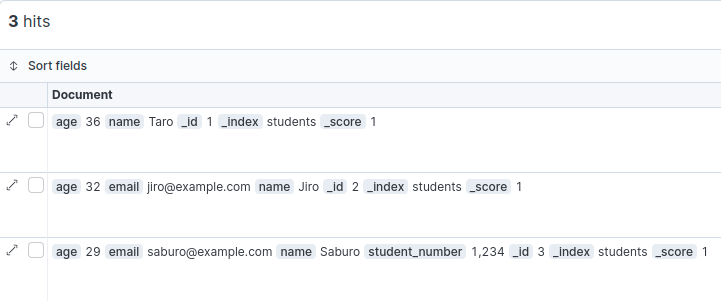
\includegraphics[width=160mm]{kibana.png}
    \caption{作成したインデックスとドキュメントをKibanaで表示したもの}
    \label{p1}
  \end{center}
\end{figure}

\section{おわりに}
今回は, 作成済みのインデックスのマッピングを更新することができることを確認した.

\begin{thebibliography}{5}
  \bibitem{1}さっと,"Python Elasticsearch 基本的な使い方まとめ",\\ https://qiita.com/satto\_sann/items/8a63761bbfd6542bb9a2,参照 May 8,2022.
  \bibitem{2}fujimotoshinji,"Elasticsearch 8.0 を docker-compose で起動する",\\ https://zenn.dev/fujimotoshinji/scraps/4fb4616976ee00,参照 May 8,2022.
\end{thebibliography}

\end{document}